\documentclass[conference]{IEEEtran}
\IEEEoverridecommandlockouts
% The preceding line is only needed to identify funding in the first footnote. If that is unneeded, please comment it out.
\usepackage{cite}
\usepackage{amsmath,amssymb,amsfonts}
\usepackage{algorithmic}
\usepackage{graphicx}
\usepackage{textcomp}
\usepackage{xcolor}
\usepackage{blindtext}
\usepackage[hidelinks]{hyperref}
\usepackage{booktabs}
\def\BibTeX{{\rm B\kern-.05em{\sc i\kern-.025em b}\kern-.08em
    T\kern-.1667em\lower.7ex\hbox{E}\kern-.125emX}}
\begin{document}

\title{COVID-19}
\author{Alexey Luchinsky \and Michael Terry  \and Vagish Vela}
\maketitle

\begin{abstract}
Goal: Compared standardized state COVID-19 datesets (including time series, county, deaths, cases, tests) with CDC provided deaths statistics for associated states to determine the increased mortality rates and potentially correlate increases in outside morbidity factors(cancer, heart disease, et cetera) as as result of state mandated lockdowns (resulting in delayed medical procedures, isolation exacerbated mental illness, et cetera).
  \blindtext
\end{abstract}

\section{Introduction}

\blindtext

\blindtext

\section{Background}

\blindtext 

\begin{eqnarray}
  \label{eq:1}
  e^{i\alpha} = \cos\alpha + i \sin\alpha
\end{eqnarray}

\blindtext 

\blindtext 

\section{Methodology}

\subsection{Ohio}
\label{Ohio}

Ohio state has a good habbit in publishing clean, tidy and very informative data. The main dataset that we will be working with, is called "COVID Summary Data" and can be found following the link \cite{system_covid-19_nodate}.

	This dataset at the current moment has more
        than 128,000 rows and discribes all the COVID- related cases in Ohio since Jan 2,2020 till the current date (Nov 18 2020). It should be noted that the dataset represents almost raw data and is in the long-table format. In total there are 9 columns in the table, representing the following fields:
        \begin{itemize}
        \item County --- County of residence
        \item Age Range --- Sex
        \item Onset Date --- Date the illness began. If onset date is unknown, the date associated with the case is used as a substitute for the date of illness onset.
        \item Date of Death --- Date of death. If date of death is unknown, this variable will be listed as “Unknown”.
        \item Admission Date --- Date of hospital admission. If the date is unknown, it will be listed as “Unknown”.
        \item Case count --- Total number of cases that meet the demographic criteria specified in the corresponding row. For example, the number in this cell is the total number of cases in a county, of the given gender, age range, onset date, etc. Each individual is only counted once. This includes both Confirmed or CDC Expanded Case Definition (Probable).
        \item Deaths Due to Illness Count --- Total number of deaths due to illness that meet the criteria in the given row. Each individual is counted once in this dataset. Note: If this cell is “0” and there is a date listed under “Date of Death” this indicates a death that was not considered to be COVID-19 related.
        \item Hospitalized Count --- Sum of hospitalizations that meet the criteria in the given row. Each individual is only counted once in this dataset. Data in this cell is cumulative and not the amount of people that are currently hospitalized.
        \end{itemize}
Typical extract from the dataset is shown on table \ref{tab:OhioDS}.


\begin{table*}
  \tiny
  \centering
  \begin{tabular}{lllllllrrr}
\toprule
{} &    County &      Sex & Age Range & Onset Date & Date Of Death & Admission Date &  Case Count &  Death Due to Illness Count &  Hospitalized Count \\
\midrule
49384  &  Hamilton &   Female &       80+ & 2020-11-19 &           NaN &            NaN &           1 &                           0 &                   0 \\
7791   &    Butler &   Female &      0-19 & 2020-11-19 &           NaN &            NaN &           1 &                           0 &                   0 \\
51824  &  Hamilton &     Male &       80+ & 2020-11-19 &           NaN &            NaN &           2 &                           0 &                   0 \\
10993  &    Butler &     Male &       80+ & 2020-11-19 &           NaN &            NaN &           1 &                           0 &                   0 \\
7588   &     Brown &     Male &       80+ & 2020-11-19 &           NaN &            NaN &           1 &                           0 &                   0 \\
7538   &     Brown &     Male &     60-69 & 2020-11-19 &           NaN &            NaN &           1 &                           0 &                   0 \\
7368   &     Brown &     Male &     20-29 & 2020-11-19 &           NaN &            NaN &           1 &                           0 &                   0 \\
7403   &     Brown &     Male &     30-39 & 2020-11-19 &           NaN &            NaN &           1 &                           0 &                   0 \\
14057  &     Clark &     Male &     70-79 & 2020-11-19 &    10/10/2020 &            NaN &           1 &                           1 &                   0 \\
121524 &     Wayne &  Unknown &      0-19 & 2020-11-19 &           NaN &            NaN &           1 &                           0 &                   0 \\
\bottomrule
\end{tabular}
\caption{Extract from Ohio dataset}
\label{tab:OhioDS}
\end{table*}

The dataset is clean. In table \ref{tab:Ohio:missing} number and percentage of the missing data in each row is shown. As you can see, we have only absent data in "admission Date" and "Date of Deaths" columns (81\% and 95\% respectively). This is not the problem of the dataset and means only that in the majority of the cases the patient was not hospitalized (and the admission date is left blank) and/or is alive (this correspond to undefined "Date of Deaths" field).

\begin{table*}[b]
  \centering
  \begin{tabular}{lll}
    \toprule
    Field Name & Missing (\%) & Comment\\
    \midrule\\
    County & 0 & \\
    Sex & 0 & \\
    Age Range & 0 & \\
               Onset Date & 0 & \\
               Date Of Death & 95 & People with missing Date of Death are still alive \\
               Admission Date &  82 & People with missing Admission Date are not hospitalized \\
               Case Count & 0 & \\
               Death Due to Illness Count & 0& \\
               Hospitalized Count & 0 & \\
    \bottomrule
  \end{tabular}
  \caption{Missing data in Ohio dataset}
  \label{tab:Ohio:missing}
\end{table*}


It was mentioned already, that the dataset is in long-table format, so a lot of information can be extracted from it after some work. For example, it is easy to construct time distributions of the total COVID cases/deaths/hospitalizations, determine the mean time spent in hospital, percentage of people died in hospitals and at home, etc. The other example of the dataset, published by COVID tracker, is available through the link \cite{covid19tracking_covid_nodate}. The data in this dataset is already processed, so only the projections of the original data (like the one doscussed earlier) on different variables are available. This makes it easier to extract some information (like time distributions of the deaths cases), but some other information (the role of age and gender, for example) is lost completely. Later in our report we will compre the results extracted from these two data sets.

The original goal of our project was to study mortality rate due to COVID and compare if with the number of deaths caused by other reasons (natural, cancer, flue, etc). On the Ohio site \cite{statistics_stats_nodate} the yearly statistics for last 4 years is presented with classification by different dearth causes. During our work we extracted this information from the site with the help of python Beautiful Soup package \cite{team_beautiful_nodate}. In table the \ref{tab:mortalityStats} current information from this site is shown. Later we have found that the same information for all states is available also in nice CSV format from the link \cite{cdc_weekly_nodate}. 

\begin{table*}
  \centering
\begin{tabular}{lrrrrr}
\toprule
Year &   2014 &   2015 &   2016 &   2017 &   Mean \\
Cause                             &        &        &        &        &        \\
\midrule
Heart Disease                     &  27000 &  28069 &  27410 &  28008 &  27621 \\
Cancer                            &  25433 &  25396 &  25509 &  25643 &  25495 \\
Accidents                         &   6178 &   6756 &   7999 &   8971 &   7476 \\
Chronic Lower Respiratory Disease &   6765 &   7211 &   7015 &   7312 &   7075 \\
Stroke                            &   5791 &   5945 &   5987 &   6425 &   6037 \\
Alzheimer’s disease               &   4083 &   4643 &   5031 &   5117 &   4718 \\
Drugs                             &   2744 &   3310 &   4329 &   5111 &   3873 \\
Diabetes                          &   3641 &   3645 &   3568 &   3740 &   3648 \\
Flu/Pneumonia                     &   2443 &   2445 &   2187 &   2243 &   2329 \\
Kidney Disease                    &   2002 &   2100 &   2262 &   2237 &   2150 \\
Septicemia                        &   1729 &   1957 &   1995 &   2066 &   1936 \\
\bottomrule
\end{tabular}
\caption{Mortality from different causes \label{tab:mortalityStats}}
\end{table*}

\subsection{Michigan}


\subsection{Indiana}






\blindenumerate[10]

\section{ Results \& Discussion }

The main goal of our project is to study the time dependence of death cases caused by COVID virus pandemic and compare it with the available data about deaths caused by other reasons (such as heart diseases, usual influencia, ect). It could be interesting also to make such an analysis for different States or even counties.

Let us start with the general yearly distributions. Unfortunately we failed to find data on natural causes statistics by county, so only state-wide analysis was performed.. It turns out that for all considered by our group states on yearly scale the COVID virus was not the main cause of death. In the case of the Ohio state, for example, it is in the 6th place, just between Alzheimer decease and strokes. (see figure \ref{fig:yearly_deaths} for more details). Almost the same situation is observed for other analyzed by our group states. In all cases heart diseases are the most important death causes, while deaths caused by COVID varus are on 4-6 place.


\begin{figure}
  \centering
  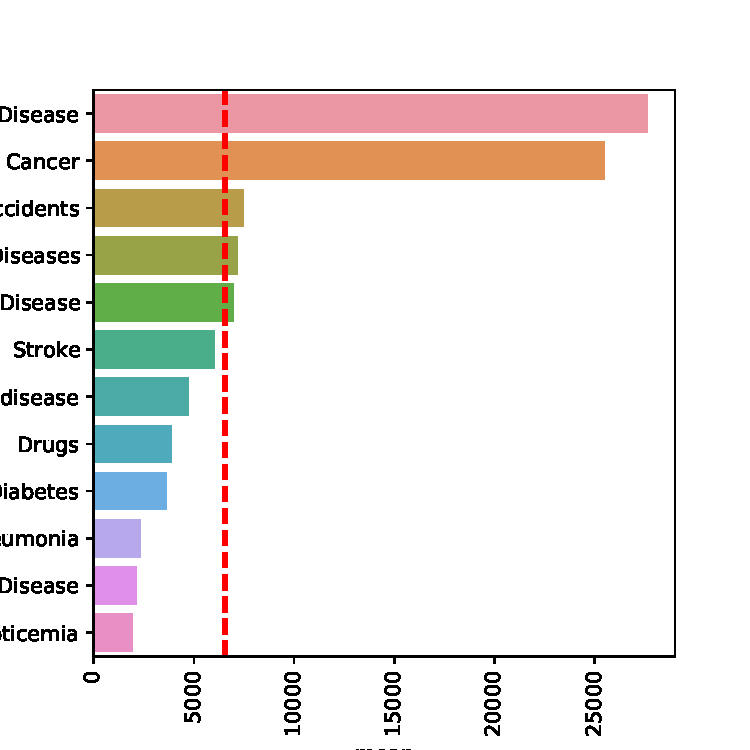
\includegraphics[width=0.9\columnwidth]{figs/yearly_deaths}
  \caption{Comparison}
  \label{fig:yearly_deaths}
\end{figure}


This point is rather interesting and seems to to be very  important. It is clear that because of various precaution measures (such as self isolation, quarantine, lockdown of different industries) the life of the whole world changed dramatically in 2020 year because of COVID a lot of necessary medical procedures were delayed or even canceled, lots of industries were almost bankrupted, etc. Not to mention the most close for us now field, i. e. the education (one can argue about some positive sides of the remote education, but it is definitely different completely from the usual face-to-face process and much more difficult for both students and instructors/professors). Thus, we can say that a lot of money and efforts were lost because of the lockdown during this pandemic and a natural question arises: does it worth it, was is really necessary? As you can see from figure \ref{fig:yearly_deaths}, heart diseases are much more dangerous, but we do not stop the life because of them.



To answer this question it could be interesting to perform a more detailed analysis and study the weekly dependence of the statistics of deaths caused by various deceases. It is clear, that COVID data, collected by our group, gives us a nice opportunity to extract time dependence of death cases with such a granularity (either directly, as for Michigan and Indiana states, or after some obvious transformations, as in the case of raw Ohio data). The same information, actually, in available from COVID-tracker project [a] , but we decided to work with the original data first. In figure \ref{fig:RT_comp_NC} we compare time distributions of the deaths cases extracted from the original data and covid-tracker results. From this figure it is clear that for all states under consideration uncumulative distributions are in good agreement, while in the case of shown in figure \ref{fig:RT_comp_CUM} cumulative results the difference is hardly noticeable.

\begin{figure*}
  \centering
  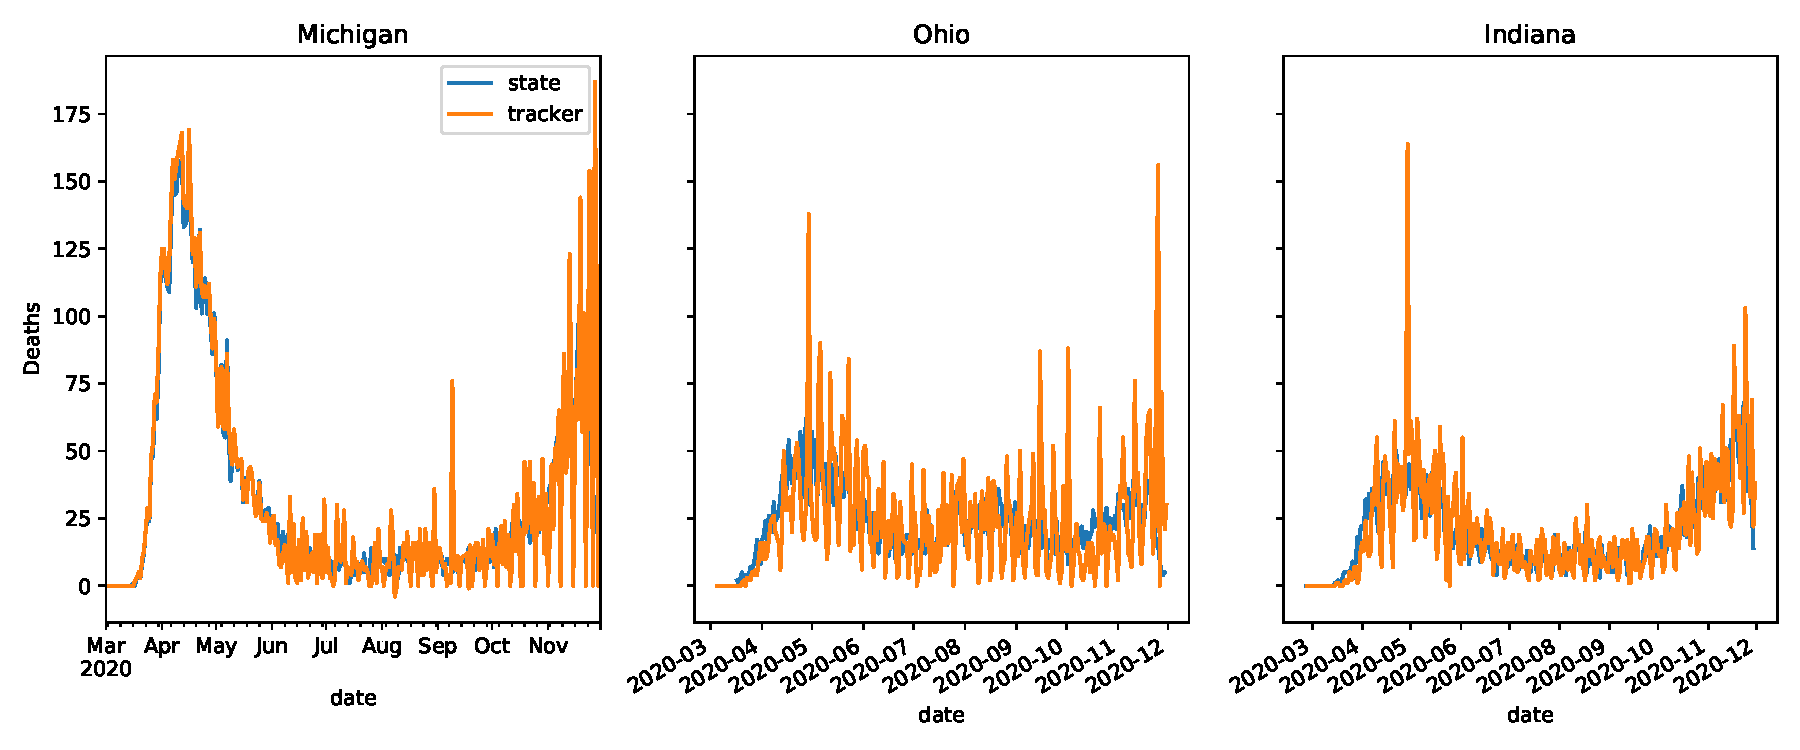
\includegraphics[width=0.9\textwidth]{figs/raw_tracker_comp_nc}
  \caption{Comparison}
  \label{fig:RT_comp_NC}
\end{figure*}

\begin{figure*}
  \centering
  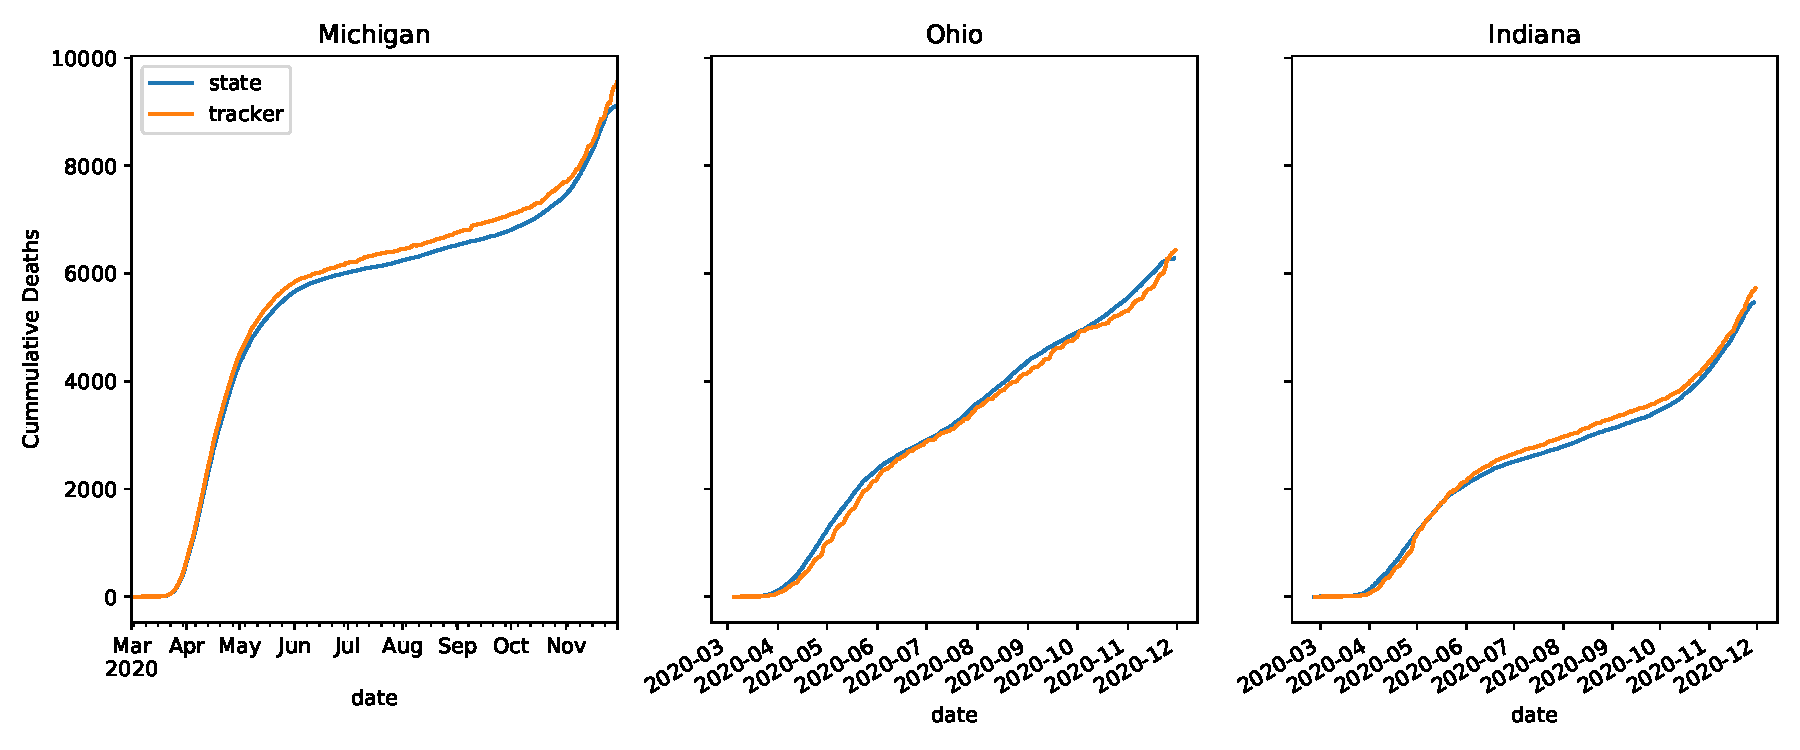
\includegraphics[width=0.9\textwidth]{figs/raw_tracker_comp_cum}
  \caption{Comparison}
  \label{fig:RT_comp_CUM}
\end{figure*}

The main results of our work are presented in figure 4. For each of the analyzed states you can see weekly distributions of death cases caused by various reasons. As you can see, for all States and for almost all time heart diseases give the main contribution to death statistics. For weeks numbers 15-25 and 45-55, however, contribution of the COVID-caused deaths is clearly seen and in some cases (Michigan state, for example) even dominant. It is clear that these two time periods correspond to two waves of the pandemic.


\begin{figure*}
  \centering
  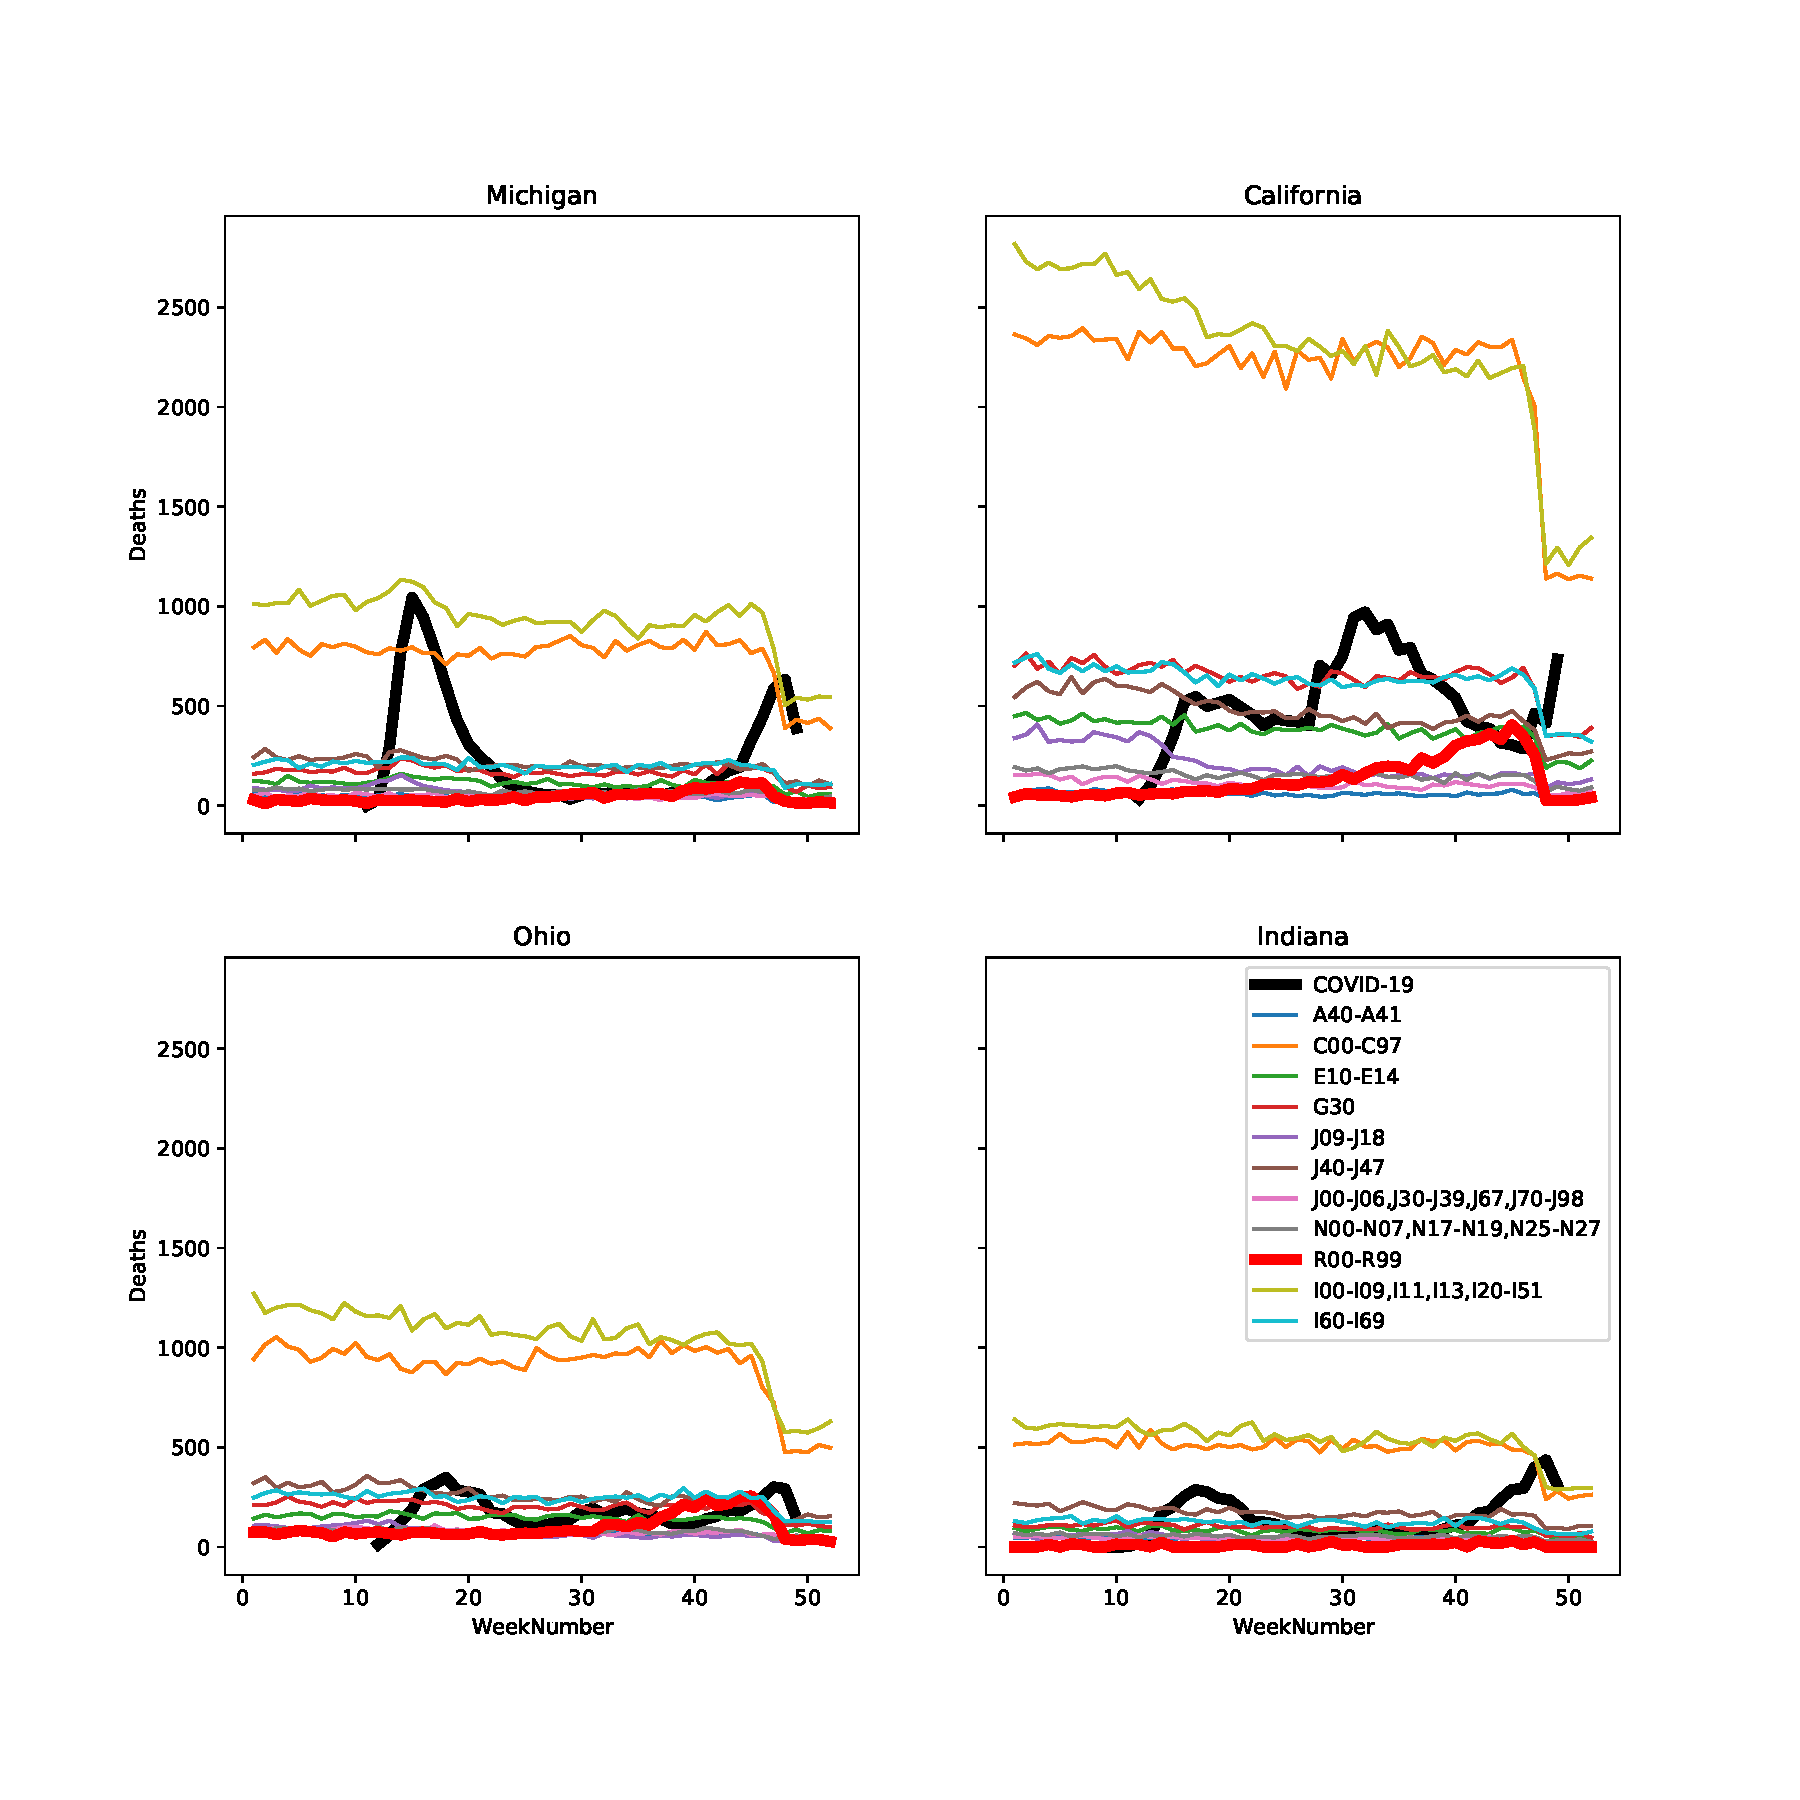
\includegraphics[width=0.9\textwidth]{figs/weekly_deaths}
  \caption{Comparison}
  \label{fig:weekly_deaths}
\end{figure*}

It could be interesting to study relative role of the virus decease in comparison with other death causes for different states and different time periods. In the case of the Michigan state, for example (see the left subfigure of figure 4) the first peak of the pandemic was devastating, the corresponding death rate was about twice as much as for heart-disease caused cases. The second peak, on the other hand is much more low. The situation is different for Ohio state: during all time period under consideration COVID-caused death rates are smaller than for two usual death reasons (heart diseases and neoplasms), but the height of the second mare is comparable with the first one. In the case of the Indiana state the situation is somewhere in the middle.

We  can make some assumptions about the reasons of such a difference. As we know, Ohio swas one of the first states that have declared the emergency situation and some of the precaution measures were taken in the stars of the panding. This results in a relatively mild first wave, but the people are too tired from the quarantine, etc, so now we have a serious second mare. In Michigan state the situation is completely different.

There is also the other interesting point in the Ohio and Michigan States data. Starting approximately from week 30 in both cases R00-R99 death cause started to gain mon weights (see zed line). According to  International Classification of Diseases scheme  \cite{ICD-10} these codes correspond to some abnormal symptoms, not elsewhere classified. We do not have enough medical education to make any definite assumptions, but such a behaviour exactly during the second wave of a new and not completely studied disease looks rather strange, we can even say suspicions.

% You can see a typical photo of our hero on figure \ref{fig}.

% \begin{figure}[htbp]
% \centerline{
\includegraphics[width = 0.9\columnwidth]{covid19.png}}
% \caption{This is it}
% \label{fig}
% \end{figure}


\section{Conclusion}

It is well known that the ending year is completely different from the others and has changed our life dramatically. we faced a lot of challenges and one of the most famous was the COVID pandemic. Although it started as a small illness in a faraway country on the other side of the ocean, pretty soon the humanity realizes that in this case the situation is very serious. Unlike rather examples (kind flue, swine flue, etc) the the mortality and the virulence of the new one is very high, it cannot be ignored and some precaution measures should be taken.

Such measures were indeed taken, different for different countries and regions. The results of such a measures also varies from countries. The quarantine was introduced throughout the world, various public gatherings and events were cancelled (Olympics 2020 in Tokyo, for example), etc. Such actions definitely helped to ease the medical side of the problem, but the other, economical issue arrises. Because of the mentioned quarantine a lot of people in the world have lost their jobs, same industries were bankrupted, etc. Moreover, since almost all medical facilities were concentrated on struggle with new decease, less was left for usual, but still important illnesen, such as heart problems, cancer, etc.

Now a natural question drises: was it worth it? We saved a lot of lifes struggling with COVID, but a lot of people died since no time and money was left for them because of this struggle. Some analysis should be made to compare all pros and contras of the current situation. This was the main question of our project.

To answer this question we have selected randomly several US States (Ohio, Michigan, Indiana) and searched for statistics of deaths caused by COVID diseases and other, usual reasons. It is clear that huge number of data can be found now concerning CONID, but we were trying to work with the original, raw data, provided by the states themselfs. Afterwards we have compared our results with the available processed data. Pretty good qualitative agreement  was observed, although some difference is also visible.

It is interesting to mention that type and quality of this "raw" data depends strongly on the state. Ohio, for example, provides the most rawest from the analyzed states. It means that some efforts should be made to extract some useful information (like time distributions, etc), while the other states give such information directly. On the other hand, the amount of information that can be extracted from the raw data is much higher, than the provided one.

The result of our work can be summarized as follows. On the first sight, if only yearly statistics of deaths is analyzed, the COVID disease does not look very dangerous: in Ohio, for example, is takes the 6th place for death causes between strokes and Alzheimer’s decease. If, however, a more detailed analysis is performed and weekly distributions are considered, the situation changed completely. In such distributions two COVID waves can be seen clearly and on the peaks of these waves the COVID caused death rates are comparable and in some states even higher the the deaths rates caused by most dangerous of the usual issued (heart attacks and cancer). So we can defenetly say that taken precaution measures were necessary. The question, however, remains wether we should leave these measures for a long time (for how long?) and  start to return to normal life.

There is one more point that is worth mentioning. In our analysis we have noticed, that in some of the states during the second COVID wave such death cause as “Abnormal symptoms, not elsewhere classified” (IDC codes \# R00-R99) take one of the leading places in the deaths statistics. In Ohio, for example, for several weeks it was in the third place (with first and second being Cancer (IDC \#C00-C97) And Chronic lower respiratory (IDC \#J40-J47) diseases.

As it was shown in the article \cite{IEEEexample:article_typical}, the night is dark and full of terrors


\bibliographystyle{IEEEtran}
\bibliography{report_litr}

\end{document}

